\newpage
\chapter{Workflow Builder}

\begin{figure}[h]
	\centering
	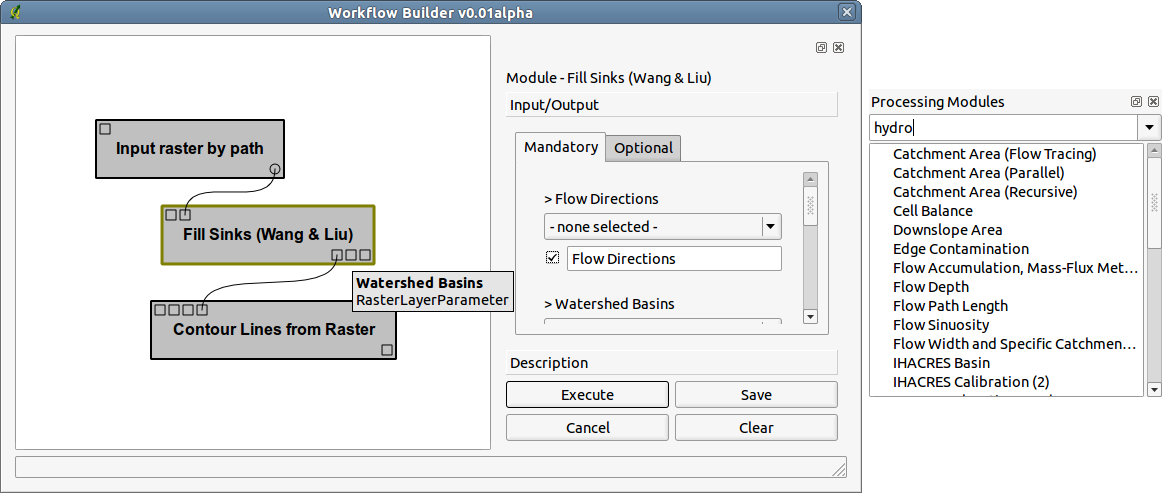
\includegraphics[scale=0.38]{pictures/wf/wf_pm}
	\caption{Workflow Builder}
  	\label{wf}
\end{figure}

Workflow Builder umožňuje uživateli propojovat moduly dostupné z QGIS
Processing Framework skrze Processing Manager. Výsledný graf (proces,
workflow) lze poté jednoduše uložit jako nový modul QGIS Processing
Frameworku. Dialogové okno Workflow Builder se skládá ze scény v levé
části, která slouží k manipulaci s moduly, propojování jejich
vstupních a výstupních parametrů pomocí myši. V panelu v pravé části
lze nastavovat hodnoty jednotlivým parametrům, které nejsou
propojeny. V pravé spodní části se nachází tlačítka pro spuštění
procesu (\textit{Execute}), k otevření dialogového okna pro uložení
procesu, pro smazání celé scény a pro schování dialogového okna
Workflow Builderu. Jakmile uživatel klikne na tlačítko pro uložení
(\textit{Save}), otevře se nové dialogové okno, kde bude vyzván k
nastavení nového modulu. Uživatel zadá jméno modulu, tagy, které
napovídají o jeho využití, popis a hlavně parametry. U parametrů může
uživatel nastavit, zdali chce, aby se parametr musel zadávat pokaždé i
v novém modulu, či hodnota bude pokaždé stejná a tudíž se nemusí ani
zobrazovat. Dále může uživatel nastavit alternativní název
parametru. Pravá spodní část dialogového okna dále obsahuje dvě
tlačítka - \textit{Cancel} a \textit{Clear}. \textit{Cancel} slouží k
schování okna a \textit{Clear} k smazání workflow, tedy všech objektů
scény.

Pro práci s Workflow Builder je dobré mít také alespoň jeden plugin,
který registruje své moduly v QGIS Processing Frameworku, dále
plugin \textbf{Workflow for Processing Framework Manager}, který byl
napsán pro načítání modulů vytvořených pomocí Workflow Builderu a
uložených do souboru ve formátu XML. Dále můžeme použít
plugin \textbf{Input parameters for WB}, který přidává do QGIS
Processing Frameworku moduly sloužící pro načítání vektorových a
rastrových dat ze souboru, které jsou následně dostupny přes výstupní
parametr daného modulu. Uživatel tedy není vázán jen na vrstvy, které
jsou načteny v QGIS.\\

Pro začátek je vhodné shlédnout instruktážní video: 
\begin{center}
	\href{http://youtu.be/4PxvWvTIyaU}{\texttt{http://youtu.be/4PxvWvTIyaU}}
\end{center}

\newpage
\newpage
\section{Tvorba workflow}
K celkovému workflow se přistupuje jako k orientovanému grafu. V tomto smyslu je graf objekt třídy \textbf{Graph} a vytvoří se při spuštění Workflow Builderu. Vrcholy představují moduly, které jsou třídy Module, a hrany představují spojení, která jsou třídy \textbf{Connection}. Do grafu se postupně přidávají moduly podle toho, jak uživatel pomocí myši přetahuje moduly z Processing Manageru. Objekt třídy Module se vytvoří na základě instance přetaženého modulu (název, popis, tagy a parametry). Modul z Workflow Builderu obsahuje parametry třídy \textbf{Port}. Instance třídy Port se také vytváří automaticky a přiřazují se danému modulu. Grafická reprezentace Module je \textbf{QGraphicsModuleItem}, který také podle \textbf{Port}ů v Module vytvoří \textbf{QGraphicsPortItem}y. Při spojování portů mezi sebou se kontroluje, zdali koresponduje typ parametru (RasterLayerParameter, NumericPrameter, ...), spojuje-li se vstupní parametr s výstupním, zdali nejsou oba parametry parametry stejného modulu a zdali není vstupní parametr prázdný (to znamená, že není spojený s jiným parametrem). Typ a název parametru můžeme zjistit posunutím myši nad parametr (čtvereček - povinný parametr, kolečko - volitelný parametr). Pakliže jsou splněny všechny podmínky, vytvoří se spojení třídy Connection a jeho grafická reprezentace \textbf{QGraphicsConnectionItem}. Connection se poté přidá do Graphu. QGraphicsConnectionItem se přidá do scény třídy \textbf{DiagramScene}, která je reimplementací třídy QGraphicsScene z knihovny Qt. Pro tvorbu spojení stačí kliknout na požadovaný vstup/výstup a táhnout myší na druhý parametr \figurename \ref{wf:crCon}.

\begin{figure}[h]
	\centering
	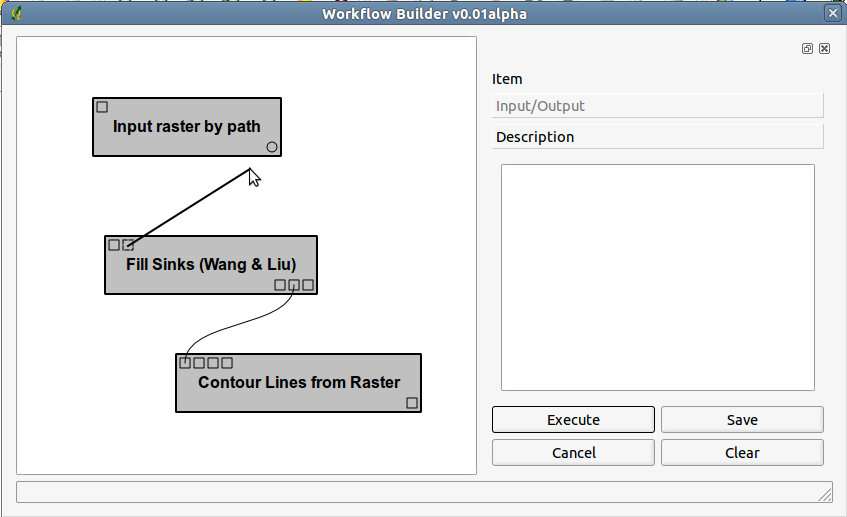
\includegraphics[scale=0.5]{pictures/wf/wf_crCon}
	\caption{Workflow Builder - tvorba spojení}
  	\label{wf:crCon}
\end{figure}

Zrušit modul či spojení můžeme tím, že si jej myší označíme a stiskneme klávesu \textit{Delete}. K mazání prvků se může také použít tlačítko $Clear$ v pravé spodní části dialogového okna, které smaže všechny prvky ve scéně včetně modulů a spojení.

V Graphu máme tedy uloženy moduly a spojení mezi nimi (Module a Connetion). Jsou uloženy jako slovníky, kde klíč je identifikační číslo modulu, resp. spojení a hodnota je instance třídy Module, resp. Connection. Ty se během tvorby workflow mění podle toho, jak uživatel přidává a odebírá moduly, spojuje je a ruší spojení.


%%%%%%
%%% postranni panel
%%%%%%
Po kliknutí na konkrétní modul se zobrazí jeho parametry v pravém postranním panelu. Ty jsou děleny na povinné a volitelné. Toto dělení, podobně jako označení výstupního parametru symbolem "$\rangle$ " před jeho název, bylo převzato z klasického dialogu pro spuštění modulu v QGIS Processing Frameworku. \\

\begin{figure}[h]
	\centering
	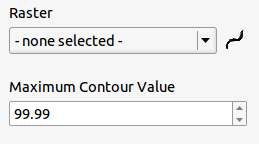
\includegraphics[scale=0.9]{pictures/wf/wf_inPar}
	\caption{Workflow Builder - vstupní parametr}
  	\label{wf:inPar}
\end{figure}

Na \figurename \ref{wf:inPar} je vidět, že widget pro nastavení vstupního parametru se skládá z jeho názvu parametru (QLabel), dále z widgetu, který se generuje na základě jeho typu (podobně jako u QGIS Processing Frameworku) a pakliže je parametr spojen s jiným, objeví se vpravo ikona signalizující spojení. \\

Widget pro nastavení výstupního parametru obsahuje řádek navíc se zaškrtávacím polem (QCheckBox) a textovým polem pro zadání názvu výstupní vrstvy (QLineEdit). Řádek slouží k načtení výstupní vrstvy  do QGIS pod uživatelem zadaným názvem, pakliže zaškrtne zaškrtávací pole. Toto mělo být pouze provizorní řešení. Workflow Builder byl testován s SAGA Pluginem a ten je v současné době napsán tak, že nerespektuje zadaný výstupní parametr a jedná-li se o vrstvu (rastrovou nebo vektorovou), vytvoří novou a tu vždy načte pod náhodně vygenerovaným názvem do QGIS. \\

\begin{figure}[!]
	\centering
	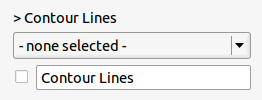
\includegraphics[scale=1.0]{pictures/wf/wf_outPar}
	\caption{Workflow Builder - výstupní parametr}
  	\label{wf:outPar}
\end{figure}


Dialogové okno Workflow Builderu spouští a ukládá workflow přes instanci třídy \textbf{Graph}. 
\newpage
\section{Spuštění workflow}
\nocite{demel:book}
Workflow se spouští tlačítkem $Execute$. Jakmile se uživatel rozhodne spustit celý proces (workflow), v grafu se vytvoří podgrafy. Ty jsou v podstatě souvislými komponentami grafu. Tvoří se rekurzivně tak, že se vytvoří podgraf třídy \textbf{SubGraph} a z prvotního seznamu všech modulů v grafu se vyjme jeden a vloží se do něj. Poté se hledají další moduly, které patří do stejné komponenty, do stejného podgrafu. Z původního seznamu všech modulů v grafu se vyjmou všechny moduly spojené s prvním modulem a uloží se do podgrafu, poté se z původního seznamu vyjmou moduly, které jsou spojené s předchozími moduly a tak dále dokud existují spojení. Zároveň se ukládají do podgrafu i spojení (instance třídy Connection). Pakliže již neexistuje další propojený modul a v původním seznamu ještě zůstali nějaké moduly, vytvoří se nový podgraf a postupuje se stejným způsobem jako u předchozího podgrafu. Jeli původní seznam modulů prázdný, znamená to, že všechny moduly z grafu jsou rozděleny do podgrafů.

Jakmile máme vytvořeny podgrafy, zjistíme, zdali je pro nás graf, resp. všechny jeho podgrafy, validní. To znamená, že se prochází každý podgraf a u každého modulu se kontroluje, zdali jsou u jeho modulů nastaveny všechny povinné vstupní parametry, případně jestli u nich existuje spojení. Pakliže se narazí na modul, u kterého není nějaký povinný vstupní parametr nastaven, uloží se do seznamu nevalidních modulů. Projdou-li se všechny moduly v podgrafu a alespoň jeden není v pořádku, není validní, vypíše se hlášení na lištu ve spodní části Workflow Builderu s informací, že některé moduly nejsou nastaveny a nemůže se pokračovat ve spouštění workflow. Zároveň se také označí moduly, o které se jedná.

Jsou-li všechny povinné vstupní parametry u všech modulů nastaveny nebo spojeny s jiným, zkontroluje se každý podgraf, zdali neobsahuje cyklus. To se provádí pomocí prohledávání grafu do hloubky [viz \lstlistingname \ref{findLoop}]. Neprojde-li kontrola, vypíše se hláška, že graf obsahuje cyklus. Projde-li kontrola a graf neobsahuje cykly, začnou se spouštět postupně všechny podgrafy. Tím zjistíme, že jsou validní a neměli by se objevit žádné známé problémy. 


\newpage
\begin{lstlisting}[label=findLoop,caption={Hledání cyklu v podgrafu},morekeywords={find}]
        def find(v):
        	# oznacim si vrchol
            v.mark = True
            eV = [seznam hran vychazejicich z vrcholu v]            
            for e in eV:
                w = e[1] # koncovy modul spojeni
                # jedna se o puvodni vrchol
                if w.id is vv.id:
                    vv.loop =  True
                    break
                # prozkoumame ho
                if not w.mark:
                    find(w)
        
        V = [seznam vrcholu v podobe Module]
        E = [seznam dvojic pocatecni a koncovy modul spojeni]

        # prochazim vrchol podgrafu
        for vv in V:
            find(vv)
            for v in V:
                v.mark = False
            if vv.loop:
            	# najdu-li cyklus
                return vv.loop

        return False
\end{lstlisting}

Samotné spouštění podgrafu začne tak, že se vezme libovolný modul z podgrafu a zkontroluje se, zdali jsou nastaveny všechny vstupy. Pakliže jsou všechny nastaveny, vytvoří se instance PF Modulu, nastaví se parametry a spustí se. Jsou-li výstupní parametry spojeny s jinými moduly, nastaví se hodnota parametru na druhém konci spojení právě získanou hodnotou. Pakliže nejsou některé vstupní parametry nastaveny, sleduje se jejich spojení a pokusí se spustit předchozí modul. Pakliže i u něho jsou nějaké parametry nenastaveny, opět se sleduje jejich spojení. Vše se opakuje do té doby, dokud se nespustí nějaký modul a ten po úspěšném provedení nastaví vstupní hodnoty v grafu následujících modulů na základě svých výstupních hodnot. Postupně se nakonec spustí všechny moduly a výstupní data se uloží. Tento proces se také řeší rekurzí.

Pozn. kontrolují se pouze vstupní parametry, protože SAGA Plugin momentálně ignoruje, zdali nastavíme výstupní parametr či ne - vytvoří si vždy nový.
\newpage
\section{Uložení workflow}
\nocite{demel:book}

K uložení nového modulu slouží tlačítko $Save$ ve spodní části
postranního panelu. Nejdříve zkontroluje, zdali graf (workflow)
neobsahuje cyklus. Je-li graf v pořádku, otevře se dialogové okno pro
nastavení informací o novém modulu. Z obrázku
[\figurename \ref{wf:saveDialog}] je vidět, že uživatel zadává jméno
modulu, tagy, popis a hlavně parametry. U nich se uživatel rozhodne,
zdali je chce v novém modulu zadávat anebo se nebudou měnit a tudíž si
nastaví jejich hodnotu při tvorbě modulu a nebude je zaškrtávat. U
parametrů, které se budou měnit, uživatel zaškrtne zaškrtávací
pole. Případně může zadat alternativní název parametru, který se mu
bude zobrazovat místo stávajícího.

\begin{figure}[h]
	\centering
	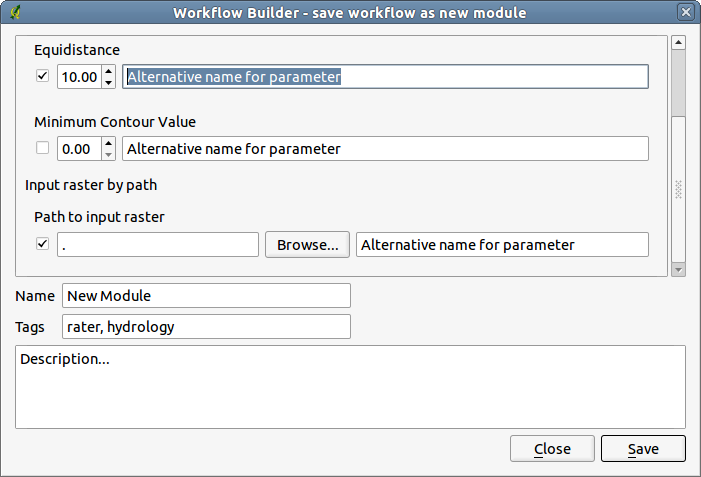
\includegraphics[scale=0.6]{pictures/wf/wf_saveDialog}
	\caption{Workflow Builder - dialog pro uložení nového modulu}
  	\label{wf:saveDialog}
\end{figure}

Po nastavení se klikne na tlačítko $Save$. Kontroluje se, zdali je
zadán název nového modulu. Nový modul se uloží jako soubor ve formátu
xml do \textbf{\$$HOME/.qgis/python/\-workflows$} s názvem stejným jako
název modulu.

\subsection{Výstupní xml souboru}
XML nabízí jednoduché uložení hierarchicky strukturovaných dat. O
prvcích XML dokumentu hovoříme jako o elementech. Elementy jsou
ohraničeny počátečními a koncovými značkami, tzv. tagy. XML dokument
obsahuje vždy právě jeden kořenový element, který se může skládat z
dalších a dalších elementů. V našem případě je kořenový element
Graph. Ten se skládá z minimálně jednoho podgrafu (SubGraph) a ten
poté minimálně z jednoho modulu (Module). Podgraf dále může obsahovat
spojení mezi moduly (Connection). Modul kromě toho obsahuje elementy
parametr (Port) a tag (tag) a také popis.  Tagy a popis jsou také
obsaženy v Grafu. \\

\begin{table}[h]
	\centering
	\begin{tabular}{|c|c|}
		\hline
                {\bf atribut} & {\bf příklad} \\
		\hline
		name & Addition two rasters \\
		tags & ['raster', 'hydrology'] \\	
		\hline	
	\end{tabular}
	\caption{Atributy elementu Graph}
	\label{tab:graph}
\end{table}

Atributy elementu více méně korespondují s atributy objektů z Workflow
Builderu. DOM reprezentace konkrétního parametru vypadá takto
[\lstlistingname \ref{portDOM}].

\begin{lstlisting}[label=portDOM,caption={příklad DOM reprezentace parametru},morekeywords={Port}]
	<Port connected="True" default_value="[]" id="944" moduleID="897"
		  name="Raster" optional="False" porttype="1" should_be_set="False" 
		  type="processing.parameters.RasterLayerParameter" value="[]">
\end{lstlisting}

\newpage
\section{Načtení workflow do PF Manageru}
Pro načtení byl napsán nový QGIS plugin \textbf{Workflow for Processing Framework Manager}, který načítá xml soubory z \$$HOME/.qgis/python/workflows$ adresáře. Na jejich základě vytvoří nové moduly, potomky processing.Module, a ty registruje v QGIS Processing Frametorku. Pro jednoduchou práci s daty uloženými v xml formátu se opět používá modul pythoní xml.dom.minidom.

Plugin načte a registruje nové moduly, když je on sám načten do QGISu. Podobně to platí i u Processing Manageru, který načte registrované moduly, když je poprvé spuštěn. Z toho plyne, že když uložíme nový modul, soubor se sice uloží, ale plugin ho hned automaticky nenačte. Aby se nový modul automaticky objevil v Processing Manageru, {\color{red}unloadnem} pluginy \textbf{Workflow for Processing Framework Manager} a \textbf{QGIS Processing Framework} a znovu je načteme. Poté opět otevřeme Processing Manager. Toto řešení je však kostrbaté.
\newpage
\section{Třídy}

O logickou část Workflow Builderu se starají třídy Graph
reprezentující graf, SubGraph reprezentující podgraf, Module
reprezentující modul, Connection reprezentující spojení a Port
reprezentující parametr modulu. Na diagramu \figurename \ref{logClass}
je znázorněný vztah po vytvoření podgrafů (souvislých komponent) v
grafu. Existuje vždy právě jedna instance třídy \textbf{Graph}. Tato
instance může obsahovat libovolné množství instancí
třídy \textbf{SubGraph}. Každá tato instance obsahuje minimálně jednu
instanci třídy \textbf{Module}, dále může obsahovat instance
třídy \textbf{Connection}. \textbf{Module} může obsahovat instance
tříd \textbf{Port}, \textbf{Connection} a právě jednu instanci
třídy \textbf{SubGraph}. Spojení v sobě drží informaci o počátečním a
koncovém parametru a modulu.

\begin{figure}[h]
	\begin{center}
		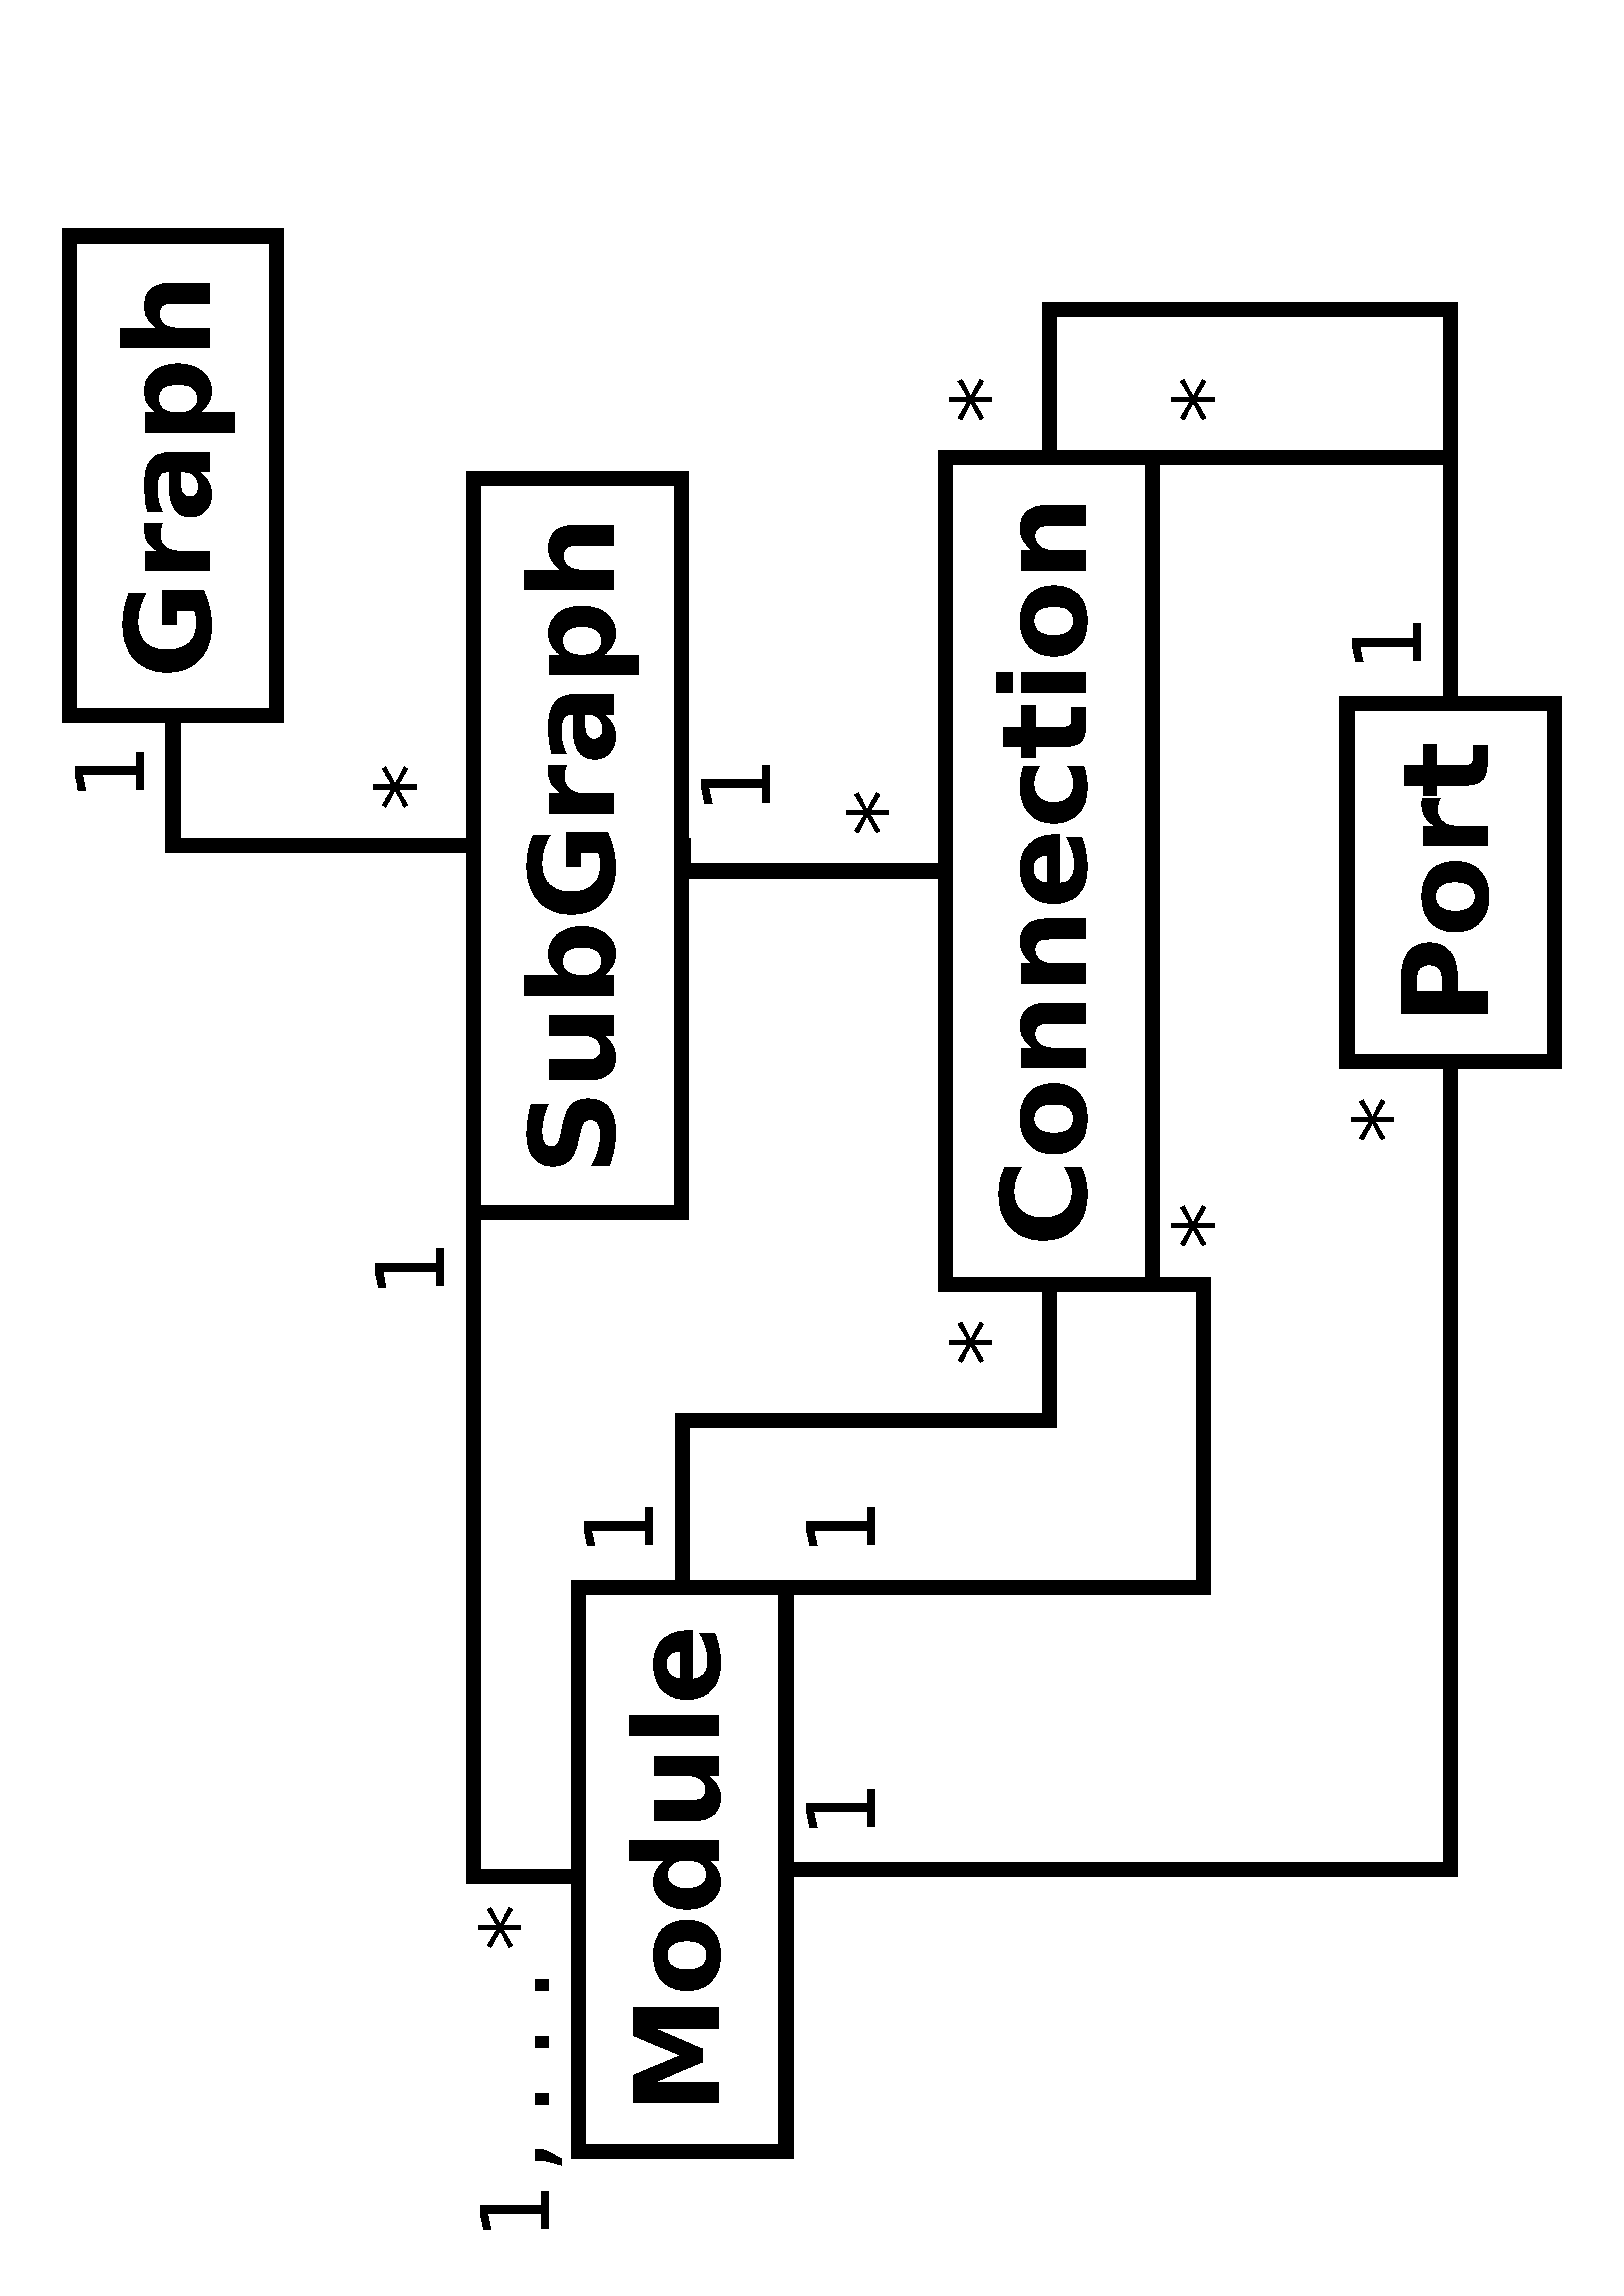
\includegraphics[scale=0.05,angle=-90]{pictures/wf/logClass.pdf}
		\caption{Diagram znázorňující vztahy mezi třídami Graph, SubGraph, Connection, Module a Port}
	  	\label{logClass}
	\end{center}
\end{figure}

Dialogové okno je instance třídy \textbf{WorkflowBuilder}, která je
potomkem třídy \textbf{QDialog} z knihovny Qt. WorkflowBuilder se
skládá z \textbf{GraphicsView} (reimplementace třídy QGraphicsView z
Qt). GraphicsView zobrazuje prvky skrze scénu (\textbf{DiagramScene} -
potomek QGraphicsScene z Qt). Třídu Module reprezentuje ve scéně
třída \textbf{QGraphicsModuleItem}, třídu Connection
třída \textbf{QGrahicsConnectionItem} a parametry jsou
reprezentovány \textbf{QGraphcisPort}.

\begin{figure}[h]
	\begin{center}
		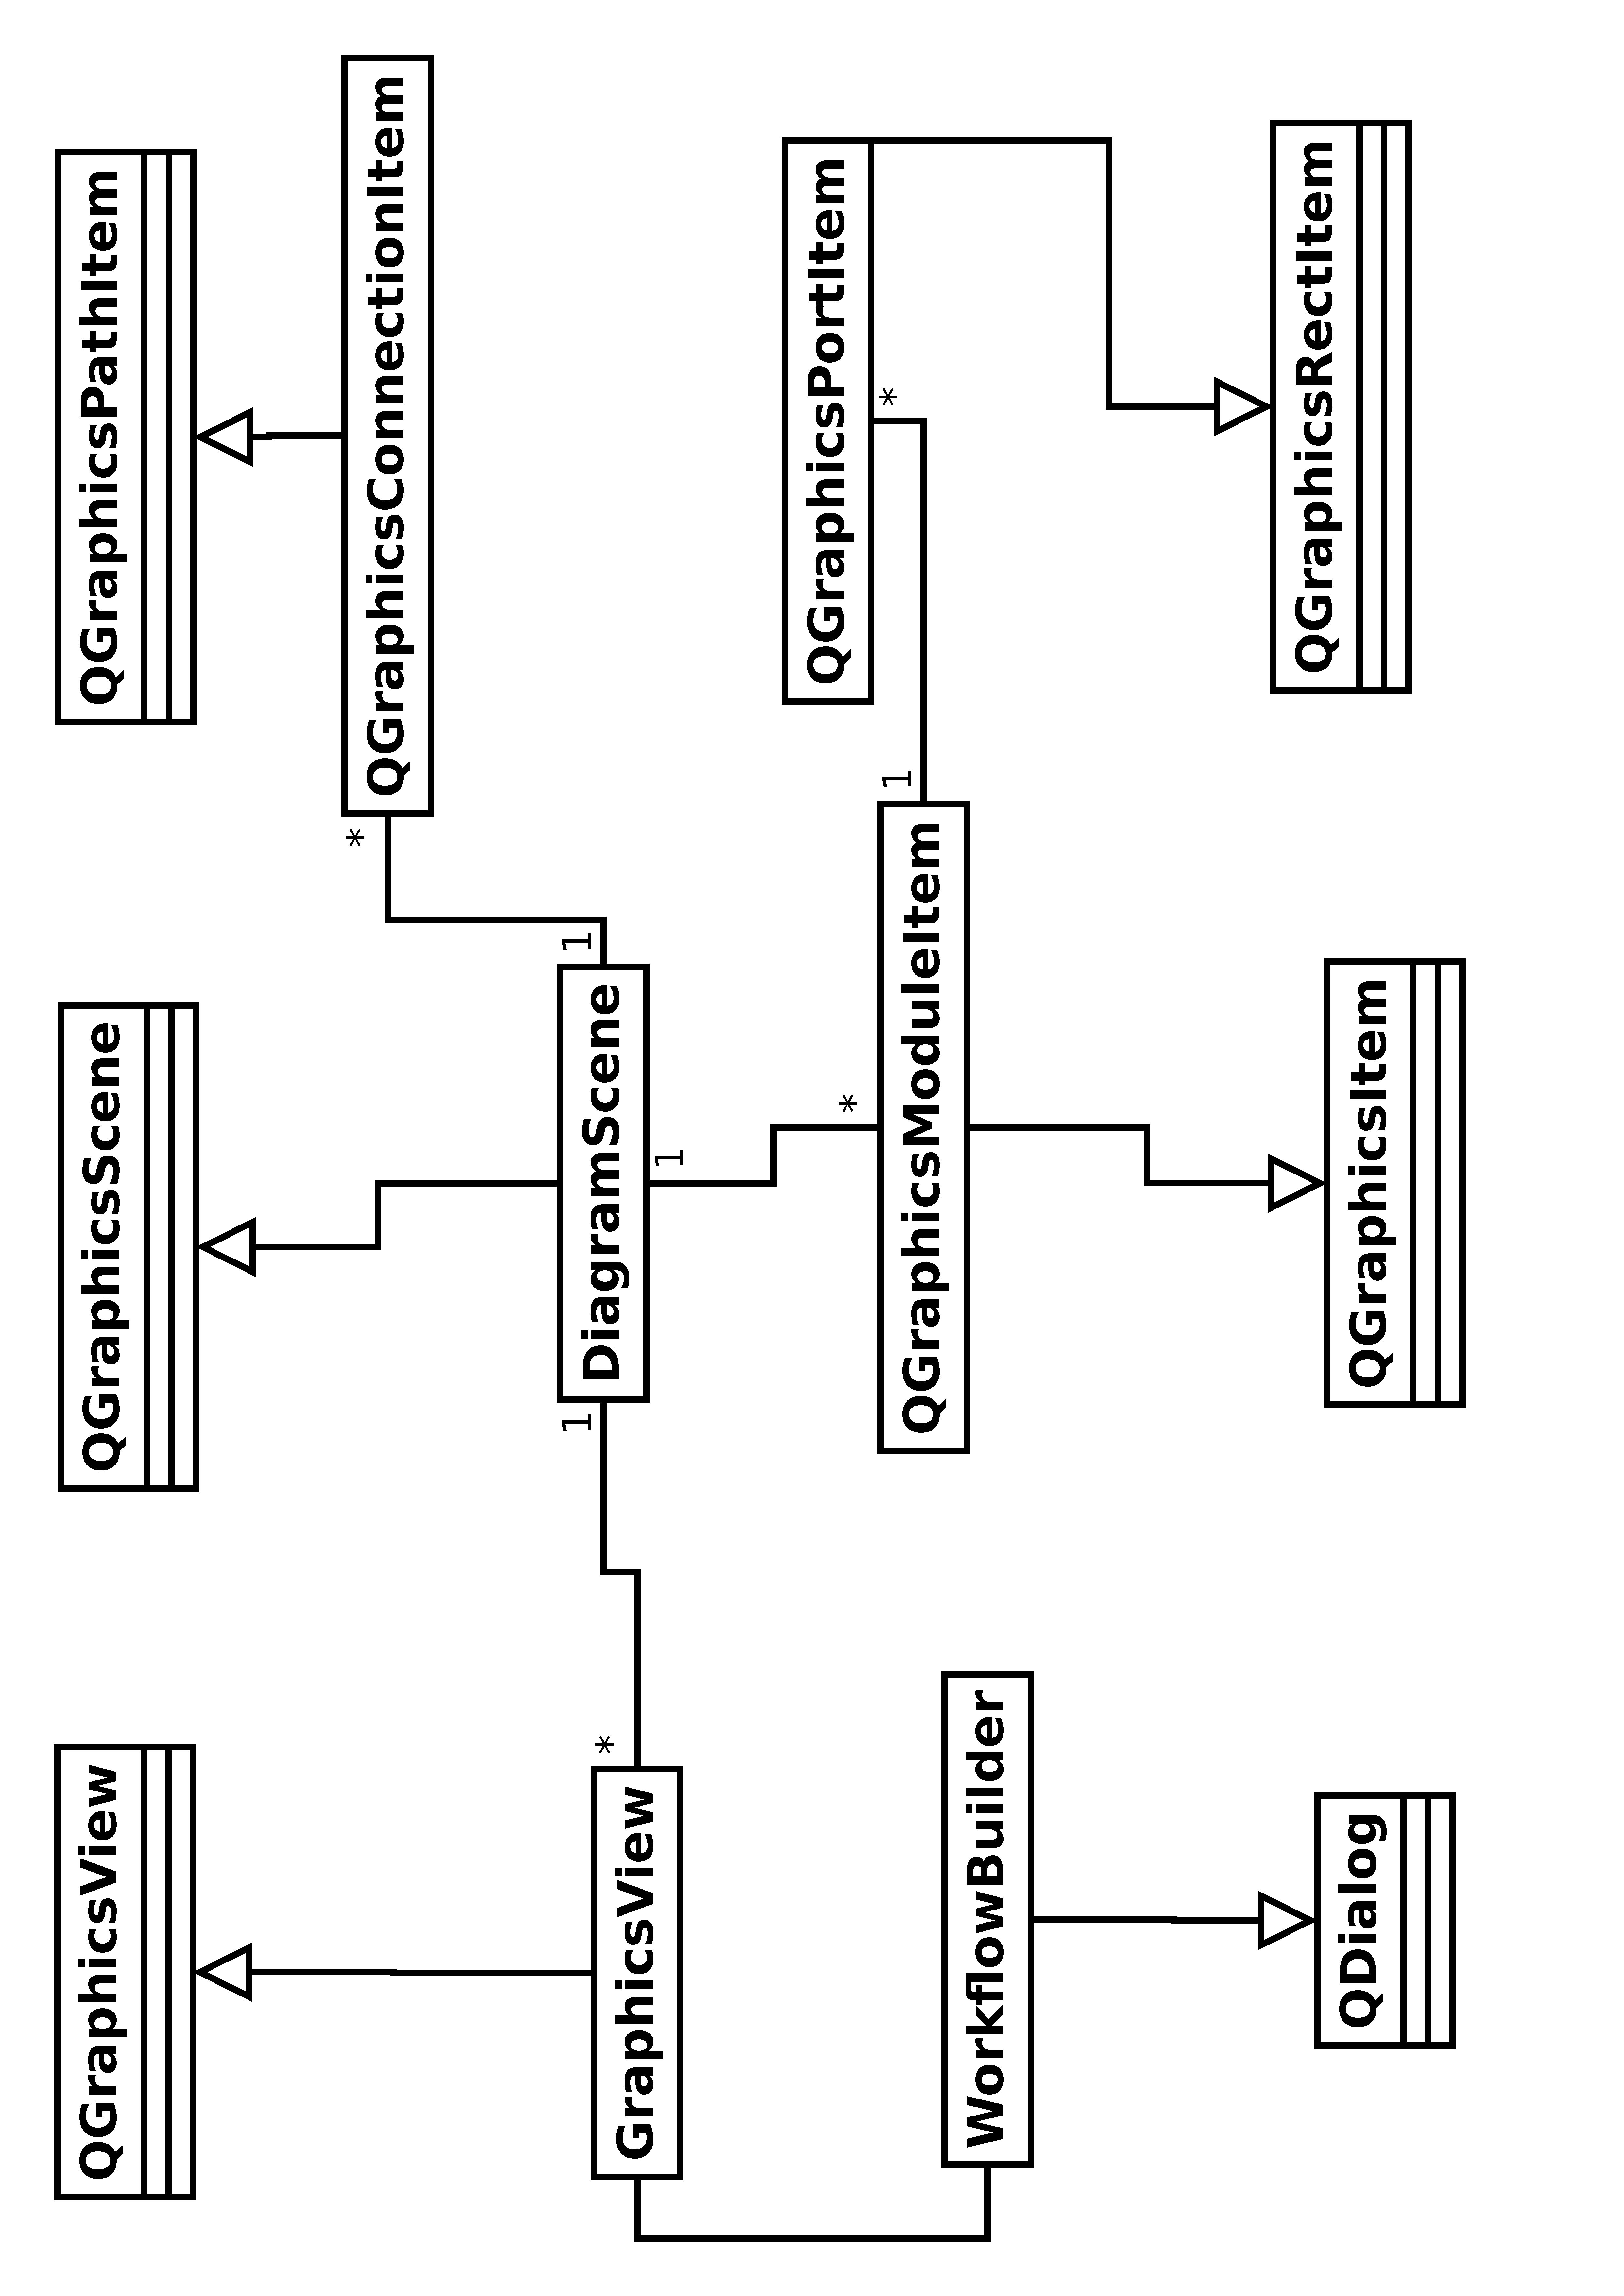
\includegraphics[scale=0.1,angle=-90]{pictures/wf/graphClass.pdf}
		\caption{Diagram znázorňující vztahy mezi třídami GraphcisView, GraphicsScene, QGraphicsModuleItem, QGraphicsConncetionItem a QGraphicsPortItem v třídě WorkflowBuilder}
	  	\label{graphClass}
	\end{center}
\end{figure}

\newpage
\subsection*{Třída Graph}
Třída Graph je v podstatě samotné workflow. Obsahuje všechny moduly a
spojení, které se ve workflow vyskytují. Hlavní metody jsou
$executeGraph$() a $save$(). Metoda $executeGraph$() postupně prochází
všechny podgrafy a jsou-li validní a neobsahují cyklus, spouští jejich
moduly. Validní podgraf je ten, u jehož každého modulu jsou všechny
vstupní parametry buď nastaveny nebo spojeny s jiným. Metoda $save$()
vytvoří xml soubor reprezentující nový modul a obsahující všechny
podgrafy, moduly a spojení. Metoda $addConnection$() přidá do grafu
spojení, $addModule$() přidá do grafu modul, $addSubGraph$() přidá do
grafu podgraf, $findLoop$() prochází graf a vrací True, najde-li v
grafu cyklus, $xml$() vytvoří DOM reprezentaci grafu.

\subsection*{Třída SubGraph}
V řeči teorie grafů instance třídy \textbf{SubGraph} reprezentují
souvislé komponenty grafu. V našem případě se jedná o instanci
třídy \textbf{Graph}, která reprezentuje workflow.

Hlavní metody jsou $executeSGraph$() a $xml$(). Metoda
$executeSGraph$() spouští všechny moduly v podgrafu. Metoda $xml$() je
důležitá při ukládání nového modulu do souboru, vytvoří DOM
reprezentaci podgrafu. Metody $prepareToExecute$() a $findLoop$() se
spouští před samotným spuštěním podgrafu. Metoda $prepareToExecute$()
prochází všechny moduly a zjišťuje, zdali jsou u každého modulu
nastaveny vstupní parametry či jsou spojeny s jiným
parametrem. Pakliže jsou, označí podgraf jako validní pomocí metody
$setValid$(). Metoda $findLoop$() slouží k nalezení cyklu v daném
podgrafu.
%processing.framework[self.label].instance()
Pomocí metod $addModule$() a $setConnections$() přidáme do podgrafu modul, resp. nastavíme spojení.

\subsection*{Třída Module}
Třída Module reprezentuje PF Module v prostředí Workflow
Builderu. Instance třídy v sobě uchovávají jméno, popis, tagy a
parametry PF Modulu. Parametry se uchovávají v podobě instance třídy
Port.

Důležité jsou metody $getInstancePF$(), $execute$() a $xml$(). Metoda
$getInstancePF$() vrací již nastavenou instanci třídy PF Module, která
koresponduje s modulem z Workflow Builderu. Pakliže u modulu ještě
nebyla vytvořena instance PF Modulu, vytvoří ji pomocí
$processing.framework[nazev\_modulu].instance()$. \textbf{Port}ům
modulu nastaví odkazy na parametry právě vytvořené instance třídy PF
Module.

Metoda $execute$() nastaví instanci PF Modulu parametru podle
aktuálních hodnot \textbf{Port}ů modulu a spustí instanci PF
Modulu. Potom nastaví hodnoty výstupů z PF Modulu do \textbf{Port}ů
modulu a dále nastaví hodnoty i u \textbf{Port}ů, které jsou s daným
výstupem (Portem, parametrem) spojené.

Metoda $xml$() vytvoří DOM reprezentaci Modulu, která slouží pro
uložení celého workflow do souboru formátu xml.

Instance třídy Module je jednoznačně identifikovatelná pomocí jejího
identifikačního čísla, které je v rámci grafu (Graph) jedinečné.

Instance třídy \textbf{Module} jsou ve scéně reprezentována instancemi
třídy \textbf{QGraphicsModelItem}.

\subsection*{Třída Port}  
Instance třídy \textbf{Port} reprezentují parametry PF Modulu. Jsou
jednoznačně identifikovatelné pomocí identifikačního čísla, které je v
rámci modulu jedinečné a pomocí identifikačního čísla modelu.

Uchovává v sobě informace jako název parametru, typ, zdali je parametr
volitelný či povinný, zdali je parametr výstupní či vstupní, popis
nebo výchozí hodnotu. Po úspěšném spuštění modulu a v případě, že
je \textbf{Port} výstup, uloží se také nová hodnota.

Pomocí metody $getValue$() získáme aktuální hodnotu, metoda
$outputData$() vrací výstupní data, $destinationPorts$() vrací porty,
které jsou s daným portem spojené a ve spojení jsou vedeny jako
cílové, $getToolTip$() vrací textový řetězec sloužící jako nápověda
pro daný port, $isConnected$() vrací zdali je daný port spojen s jiným
a $xml$() vrací DOM reprezentaci portu. Je-li \textbf{Port} výstupní,
pomocí metody $addItToCanvas$() zjistíme, zdali si uživatel přál
načíst vrstvu po spuštění modulu do QGIS, a metoda $outputName$() nám
vrátí jméno, pod kterým se má vrstva načíst.

Instance třídy \textbf{Port} jsou ve scéně reprezentovány instancemi
třídy \textbf{QGraphicsPortItem}.

\subsection*{Třída Connection}
Třída \textbf{Connection} v terminologii teorie grafů reprezentuje
hrany. Uchovává v sobě informaci o počátečním a koncovém modulu
(Module), resp. parametru (Port). A obsahuje jedinou metodu xml(),
která vrací DOM reprezentaci spojení.

Instance třídy \textbf{Connection} jsou ve scéně reprezentovány
instancemi třídy \textbf{QGraphicsConnectionItem}.

\subsection*{Třída GraphicsView}
Třída \textbf{GraphicsView} je reimplementací
třídy \textbf{QGraphicsView} z knihovny Qt. Byla reimplementována
metoda $wheelEvent$(), která umožňuje funkci zoom, a metody
$dragEnterEvent$(), $dragMoveEvent$() a $dropEvent$() pro spravování
událostí týkajících se prostředí Drag and Drop. \textbf{GraphicsView}
přijímá pouze objekty z Processing Manageru. Metoda $keyPressEvent$()
je reimplementována tak, aby se po stisknutí klávesy $Delete$ smazaly
všechny vybrané prvky.


\subsection*{Třída DiagramScene}
Třída \textbf{DiagramScene} je reimplementací
třídy \textbf{QGraphicsScene} z knihovny Qt. Byly reimplementovány
metody \textit{mousePressEvent}(), \textit{mouseMoveEvent}()
a \textit{mouseReleaseEvent}(). Tyto metody řeší, zdali uživatel pouze
kliknul na modul a chce, aby se mu zobrazili informace o parametrech,
či kliknul na parametr a chce jej spojit s jiným. Také se zde řeší,
zdali mohou být parametry spojeny. Pakliže ano, vytvoří se spojení
(instance třídy Connection) a na jeho základě také instance
třídy \textbf{QGraphicsConnection}.

Pomocí metod \textit{addModule}(processing.Module) se vytvoří nejdříve
Objekt třídy Module a na jeho základě
objekt \textbf{QGraphicsModuleItem}. Metoda \textit{delModule}() maže
modul ze scény (DiagramScene) i z grafu (Graph) a zároveň i jejich
spojení s druhými moduly. Metoda \textit{delConnection}() maže spojení
ze scény (DiagramScene) i z grafu (Graph).

Metoda \textit{clearDockPanel}() smaže informace z pravého postranního
panelu.

